% Copyright (C) 2007 Technical University of Liberec.  All rights reserved.
%
% Please make a following reference to Flow123d on your project site if you use the program for any purpose,
% especially for academic research:
% Flow123d, Research Centre: Advanced Remedial Technologies, Technical University of Liberec, Czech Republic
%
% This program is free software; you can redistribute it and/or modify it under the terms
% of the GNU General Public License version 3 as published by the Free Software Foundation.
%
% This program is distributed in the hope that it will be useful, but WITHOUT ANY WARRANTY;
% without even the implied warranty of MERCHANTABILITY or FITNESS FOR A PARTICULAR PURPOSE.
% See the GNU General Public License for more details.
%
% You should have received a copy of the GNU General Public License along with this program; if not,
% write to the Free Software Foundation, Inc., 59 Temple Place - Suite 330, Boston, MA 021110-1307, USA.
%
%%%%%%%%%%%%%%%%%%%%%%%%%%%%%%%%%%%%%%%%%%%%%%%%%%%%%%%%%%%%%%%%%%
%
% use PDFLatex to compile this
%

\documentclass[a4paper]{article}
\usepackage{authblk}
%\usepackage{rotating}
%\usepackage{pdflscape}

\usepackage[bbgreekl]{mathbbol}
\usepackage{amssymb, amsmath, amsthm, stmaryrd}

\usepackage{array}
\usepackage{longtable}
\usepackage[usenames,dvipsnames]{color}   %colors
%\usepackage{colortbl}   %colorful tables
\usepackage{tabularx,tikz}
\usepackage{graphicx} %[dvips]
% it is note used \usepackage{cooltooltips}

%these two can be found in caption package
%\usepackage{caption}
%\usepackage{subcaption}

\usepackage[numbers]{natbib}
\usepackage{ulem}
\usepackage{etoolbox}
\usetikzlibrary{arrows,matrix}


%%%%%%%%%%%%%%%%%%%%%%%%%%%%%%%%%%%%%%%%%%%%%%%%%%%%%%%%%%%%%%%%%%%%%%%%%%%%
\newtheorem{theorem}{Theorem}
\newtheorem{corollary}[theorem]{Corollary}
\newtheorem{lemma}[theorem]{Lemma}

%%%%%%%%%%%%%%%%%%%% specific math macros
\def\abs#1{\lvert#1\rvert}
\def\Abs#1{\bigl\lvert#1\bigr\rvert}
\def\adiv{\widetilde\div}
\def\aep{\tilde\ep}
\def\agrad{\widetilde\nabla}
\def\avg#1{\left\{\mskip-5mu\left\{#1\right\}\mskip-5mu\right\}}
\def\CC{\tn C}
\def\d {\,{\rm d}}
\def\ddt#1{\frac{\d #1}{\d t}}
\def\dist{\operatorname{dist}}
\def\div{\operatorname{div}}
\def\dn{\d\nnu}
\def\dt{\prtl_t}
\def\dual#1#2{\left\langle #1,#2\right\rangle}
\def\ee{\vc e}
\def\ep{\vc\varepsilon}
\def\FF{\vc F}
\def\ff{\vc f}
\def\grad{\nabla}
\def\Hel{\vc{\mathcal H}}
\def\Hf{\mathcal H}
\def\jmp#1{\left\llbracket #1 \right\rrbracket}
\def\Lapl{\Delta}
\def\Natural{\mathbf N}
\def\nn{\vc n}
\def\nnu{\vc\nu}
\def\norm#1{\left\|#1\right\|}
\def\ol{\overline}
\def\pbar{\overline p}
\def\pphi{{\varphi}}
\def\prtl{\partial}
\def\qq{\vc q}
\def\Real{{\mathbf R}}
\def\tn#1{{\mathbb{#1}}}    % tensor
\def\tr{\operatorname{tr}}
\def\tt{\vc t}
\def\U{\vc U}
\def\ubar{\overline\uu}
\def\ul{\underline}
\def\uu{\vc u}
\def\V{\vc V}
\def\Vel{{\vc{\mathcal V}}} % Sobolev space for elasticity
\def\Vf{{\mathcal V}} % Sobolev space for flow
\def\vc#1{\mathbf{\boldsymbol{#1}}}     % vector
\def\vv{\vc v}
\def\weakly{\rightharpoonup}
\def\xx{\vc x}
\def\yy{{\vc y}}

\newcommand{\eq}[1]{\begin{equation}#1\end{equation}}
\newcommand{\ml}[1]{\begin{multline}#1\end{multline}}
\newcommand{\mls}[1]{\begin{multline*}#1\end{multline*}}

\newcommand{\note}[2]{{\color{blue} \textbf{ #1:} \textit{#2}}}
%% ini_table members
%%%%%%%%%%%%%%%%%%%% specific math macros

\newcommand{\opm}{ % plus and minus in circle
  {\mathbin{
    \mathchoice
      {\buildcirclepm{\displaystyle     }{0.14ex}{0.95}{0.05ex}{.7}}
      {\buildcirclepm{\textstyle        }{0.14ex}{0.95}{0.05ex}{.7}}
      {\buildcirclepm{\scriptstyle      }{0.13ex}{0.955}{0.04ex}{.55}}
      {\buildcirclepm{\scriptscriptstyle}{0.08ex}{0.95}{0.03ex}{.45}}
  }} 
}
\newcommand\buildcirclepm[5]{%
  \begin{tikzpicture}[baseline=(X.base), inner sep=-#5, outer sep=-.65]
    \node[draw,circle,line width=#4] (X)  {\footnotesize\raisebox{#2}{\scalebox{#3}{$#1\pm$}}};
  \end{tikzpicture}%
}


%%%%%%%%%%%%%%%%%%%%%%%%%%%%%%%%%%%%%%%%%%%%%%%%%%%%%%%%%%%%%%%%%%%%%%%%%%%%%%%%%%%%%%%%%%%%% BEGIN DOCUMENT
\begin{document}

\title{Mixed-dimensional models of linear elasticity and poroelasticity}
\author{Jan Březina}
\author{Jan Stebel}
\affil{Technical University of Liberec,\\ Studentská 1402/2, 461 17 Liberec, Czech Republic}
\affil{e-mail: \texttt{\{jan.brezina,jan.stebel\}@tul.cz}}
\maketitle


\section{Introduction}

In this paper we describe a dimension reduction for the Biot system of poroelasticity in a domain containing a fracture, which is assumed to be a thin manifold around a subset of hyperplane.
The obtained equations (eq. \eqref{eq:lin_el_frac}, \eqref{eq:flow_frac}) are expressed in terms of mean pressure and mean displacement in the fracture.
The resulting problem consists of equations of flow and mechanics in the fracture and in the surrounding domain, accompanied by appropriate interface conditions (eq. \eqref{eq:interface_el}, \eqref{eq:interface_flow}).
Finally we analyse the well-posedness of the steady-state mechanical part of the problem.

The original idea of dimension reduction comes from \cite{martin_modeling_2005}, where it was applied to the darcian flow model.
Here we also deal with the linear elasticity system, for which the approach has to be generalized using tangential and normal calculus in the fracture.

The structure of the paper is as follows.
In section \ref{sec:model} we describe the original mathematical model and the full and reduced geometry.
The tangential and normal calculus is presented in section \ref{sec:calculus}.
In sections \ref{sec:reduction_elasticity} and \ref{sec:reduction_flow} we derive the reduced problem for mechanics and flow, respectively.
Finally, in section \ref{sec:wellposedness_elasticity} we prove the existence and uniqueness of weak solution to the mechanical part of the resulting problem.


\section{Biot's poroelasticity in domain with fracture}\label{sec:model}

\begin{figure}[h]
\centering
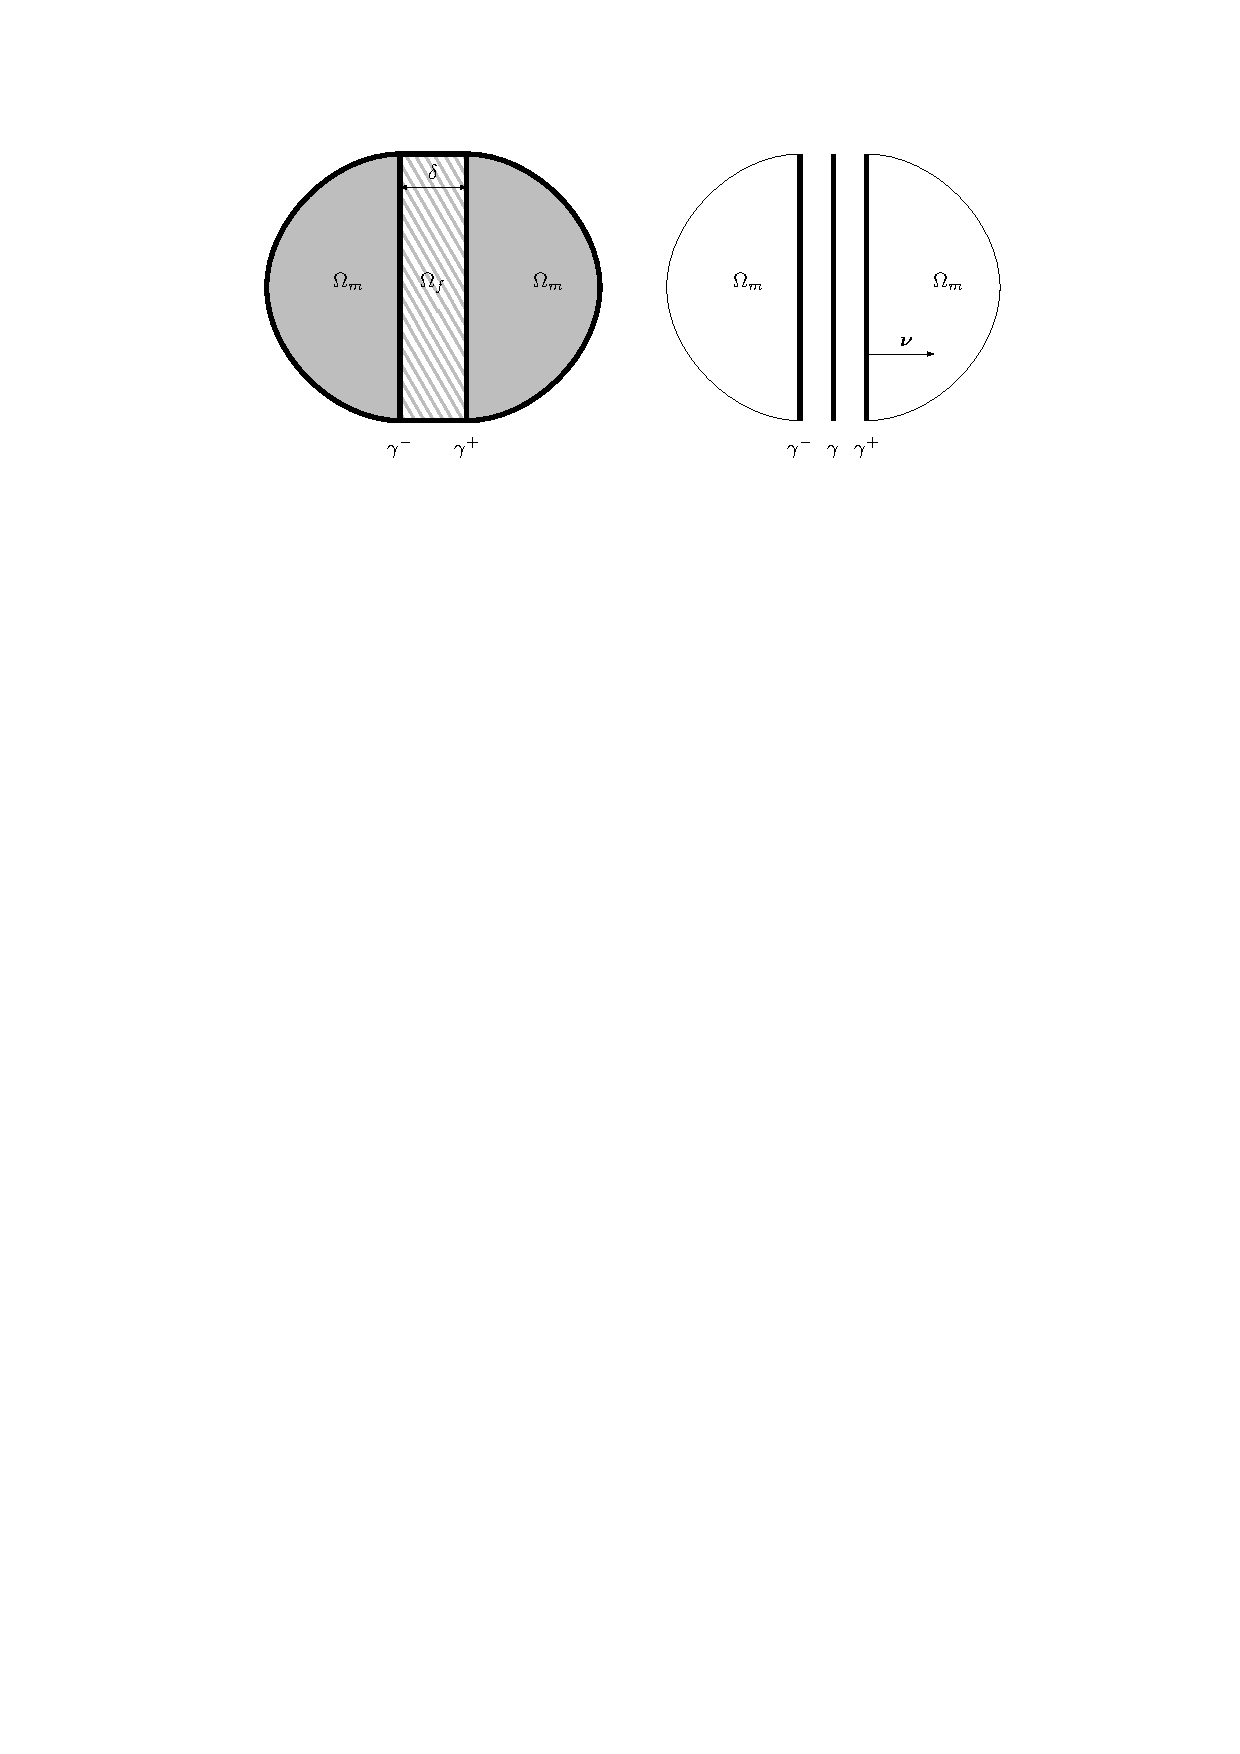
\includegraphics[width=\textwidth]{figures/omegas}
\caption{The domain of the full model (left) and the reduced geometry (right).}
\label{fig:omegas}
\end{figure}

Let $\Omega$ be a bounded, simply connected domain in the Euclidean space $\Real^d$, $d\in\{2,3\}$, with Lipschitz boundary $\partial\Omega$.
We assume that $\Omega$ is composed of two subdomains: the fracture $\Omega_f$ and the matrix $\Omega_m:=\Omega\setminus\overline\Omega_f$.
The matrix is assumed to be divided into two parts (see Figure \ref{fig:omegas}).
For simplicity we consider straight fracture, i.e. there is a subset $\gamma$ of a hyperplane in $\Real^d$ and a number $\delta>0$ so that
\eq{ \Omega_f = \{\xx+s\nnu;~\xx\in\gamma,~s\in(-\tfrac\delta2,\tfrac\delta2)\}, }
where $\nnu$ stands for the unit normal vector to $\gamma$.
The parameter $\delta$ is usually called the aperture or the width of the fracture.

Without loss of generality we can take $\gamma:=\Omega\cap\left(\{0\}\times\Real^{d-1}\right)$ and $\nnu:=(1,0,0)^\top$.
Then the two parts of $\Omega_m$ are interacting with $\Omega_f$ via the interfaces
\eq{ \gamma^+:=\Omega\cap\big( \{\tfrac\delta2\}\times \Real^{d-1}\big), \quad \gamma^-:=\Omega\cap\big( \{ -\tfrac\delta2\}\times \Real^{d-1}\big). }
The symbol $\prtl\gamma$ shall denote the relative boundary of $\gamma$.

% We shall derive a model of poroelasticity on the reduced geometry consisting of $\Omega_m$ and $\gamma$.
The basic hydro-mechanical interaction in a porous media is described by the Biot system of poroelasticity.
In context of this paper it reads:
\begin{subequations}
\label{eq:biot}
\begin{align}
    \label{eq:lin_el}
    -\div \bbsigma + \nabla(\alpha p) &= \ff &&\mbox{ in }\Omega_m\cup\Omega_f,\\
\label{eq:biot_darcy}    \dt\left(Sp + \div(\alpha\uu)\right) + \div\qq &= g &&\mbox{ in }\Omega_m\cup\Omega_f,
\end{align}
\end{subequations}
Here, the displacement $\uu$ and the pressure $p$ are the principal unknowns; further $\alpha$ is the Biot effective stress parameter, $\ff$ the body force, $S$ the storativity, $g$ the fluid source.
The stress tensor $\bbsigma$ is given by the Hooke law:
\eq{ \bbsigma = \CC\nabla\uu, }
where $\CC$ is the $4^{\rm th}$-order elasticity tensor, and the flux $\qq$ is given by the Darcy law:
\eq{ \quad \qq = -\tn K\nabla p }
via the hydraulic conductivity tensor $\tn K$.
To complete the equations in $\Omega$, we require that
\eq{ \label{eq:continuity_on_gamma_pm} p,\uu,\qq\cdot\nnu,\bbsigma\nnu \mbox{ are continuous on } \gamma^\pm. }

In what follows, we shall assume that the physical parameters $\alpha,S,\CC,\tn K$ are constant in $\Omega_m$, $\Omega_f$, respectively.
To distinguish values in $\Omega_m$ and $\Omega_f$, we shall use the subscripts ``$m$'' and ``$f$'', i.e. $\alpha_m := \alpha_{|\Omega_m}$, $\alpha_f := \alpha_{|\Omega_f}$ etc.
In addition, it is assumed that $\CC_*$ and $\tn K_*$, $*\in\{m,f\}$, have the usual symmetries:
\eq{ \label{eq:sym_C} \forall \tn A,\tn B\in\Real^{d\times d}:~ \CC_*\tn A:\tn B=\CC_*\tn A^\top:\tn B=\CC_*\tn A:\tn B^\top=\CC_*\tn B:\tn A, }
\eq{ \tn K_* = \tn K_*^\top, }
and are positive definite in the following sense:
There exist positive constants $\mu_m$, $\mu_f$, $\lambda_m$, $\lambda_f$, $\kappa_m$, $\kappa_f$, such that
% \eq{ \label{eq:pos_def_C} \forall\tn A\in\Real^{d\times d}_{sym}:~\CC_*\tn A:\tn A \ge C_1|\tn A|^2, }
\eq{ \label{eq:pos_def_C_gen} \forall\tn A\in\Real^{d\times d}:~\CC_*\tn A:\tn A \ge \mu_*\left|\tn A+\tn A^\top\right|^2 + \lambda_*|\tn I:\tn A|^2, }
\eq{ \label{eq:pos_def_K} \forall\vv\in\Real^d:~\tn K_*\vv\cdot\vv \ge \kappa_*|\vv|^2,\quad *\in\{m,f\}. }
Here %$\Real^{d\times d}_{sym}$ stands for the set of symmetric $d\times d$ matrices and 
$|\tn A|$ denotes the Frobenius norm, i.e. $|\tn A|^2=\tn A:\tn A$.
% It is not difficult to observe that \eqref{eq:sym_C} and \eqref{eq:pos_def_C} imply:
% \eq{ \label{eq:pos_def_C_gen} \forall\tn A\in\Real^{d\times d}:~\CC_*\tn A:\tn A \ge C_1\left|\frac{\tn A+\tn A^\top}2\right|^2. }
% A further natural requirement is that $\nnu$ is an eigenvector of $\tn K_f$, i.e.
% \eq{\label{eq:normal_conductivity} \tn K_f\nnu = k_f\nnu, }
% where $k_f>0$ is the hydraulic conductivity in orthogonal direction to $\gamma$.




\section{Tangential and normal calculus in fracture}\label{sec:calculus}

Let $\tn P := \nnu\otimes\nnu$ be the orthogonal projector to $\gamma$.
For any $\vv\in\Real^d$ and $\tn A\in\Real^{d\times d}$ we shall define the orthogonal decomposition into normal and tangential direction to $\gamma$:
\eq{ \vv = \tn P\vv + (\tn I-\tn P)\vv =:\vv_\nu + \vv_\tau, }
\eq{ \tn A = \tn A\tn P + \tn A(\tn I-\tn P) =: \tn A_\nu + \tn A_\tau. }
Likewise we decompose differential operators acting on vector- and tensor-valued functions:
\eq{ \label{eq:grad_sc} \nabla f = (\nabla f)_\nu + (\nabla f)_\tau =: \nabla_\nu f + \nabla_\tau f, }
\eq{ \label{eq:grad_vc} \nabla\vv = (\nabla\vv)_\nu + (\nabla\vv)_\tau =: \nabla_\nu\vv + \nabla_\tau\vv, }
\eq{ \div\vv = \div\vv_\nu + \div\vv_\tau =: \div_\nu\vv + \div_\tau\vv, }
\eq{ \label{eq:div_tn} \div\tn A = \div(\tn P\tn A) + \div((\tn I-\tn P)\tn A) =: \div_\nu\tn A + \div_\tau\tn A. }
Here $[\nabla\vv]_{ij}=\tfrac{\prtl v_i}{\prtl x_j}$ and $[\div\tn A]_j = \sum_{i=1}^d\tfrac{\prtl a_{ij}}{\prtl x_j}$.
Let $w$ be a function defined in $\gamma^+$ and $\gamma^-$.
Shifting its argument to $\gamma$, we obtain new functions $w^\oplus$, $w^\ominus$ defined in $\gamma$ as follows:
\eq{ w^{\opm}(\xx) := w(\xx\pm\tfrac\delta2\nnu), ~\xx\in\gamma. }
Now we can introduce the average and the jump operator:
\eq{ \avg{w} := \frac{w^\oplus+w^\ominus}2,\quad \jmp{w} := w^\oplus-w^\ominus. }
When integrating across the fracture, we shall write
\[ \int w\dn := \int w(\cdot+s\nnu)\d s. \]
The symbol $\overline w$ will denote the integral mean of $w$ across the fracture aperture, i.e.
\eq{\label{eq:def_mean} \overline w(\xx):=\frac1\delta\int_{-\tfrac\delta2}^{\tfrac\delta2} w(\xx) \dn,~\xx\in\gamma. }
Then, for all sufficiently smooth functions $f$, $\vv$ and $\tn A$ defined in $\Omega_f$ it holds:
\eq{ \label{eq:int_grad_nu_sc}
\int_{-\tfrac\delta2}^{\tfrac\delta2}\nabla_\nu f\dn = \int_{-\tfrac\delta2}^{\tfrac\delta2}\nnu\frac{\rm d}{{\rm d}s}\left(f(\cdot+s\nnu)\right)\d s = \jmp{f}\nnu,
}
\eq{ \label{eq:div_nu_vc}
\int_{-\tfrac\delta2}^{\tfrac\delta2}\div_\nu\vv\dn = \int_{-\tfrac\delta2}^{\tfrac\delta2}\nnu\cdot\frac{\rm d}{{\rm d}s}\left(\vv(\cdot+s\nnu)\right)\d s = \jmp{\vv}\cdot\nnu,
}
\eq{ \label{eq:int_grad_nu_vc} \int_{-\tfrac\delta2}^{\tfrac\delta2}\nabla_\nu\vv\dn = \jmp{\vv}\otimes\nnu, }
\eq{ \label{eq:int_div_nu_tn} \int_{-\tfrac\delta2}^{\tfrac\delta2}\div_\nu\tn A \dn = \jmp{\tn A^\top}\nnu. }
Motivated by the above identities, we introduce the approximate gradient and divergence operators in the positive and negative half of fracture:
\eq{ \agrad^\opm[f,\overline f] := \nabla_\tau\overline f \pm \frac2\delta(f^\opm - \overline f)\nnu, }
\eq{ \agrad^\opm[\vv,\overline\vv] := \nabla_\tau\overline\vv \pm \frac2\delta(\vv^\opm - \overline\vv)\otimes\nnu, }
\eq{ \adiv^\opm[\vv,\overline\vv] := \div_\tau\overline\vv \pm \frac2\delta(\vv^\opm - \overline\vv)\cdot\nnu, }
\eq{ \adiv^\opm[\tn A,\overline{\tn A}] := \div_\tau\overline{\tn A} \pm \frac2\delta(\tn A^\opm - \overline{\tn A})^\top\nnu, }
which satisfy:
\eq{\label{eq:agrad} \avg{\agrad[f,\overline f]} = \overline{\nabla f}, \quad \avg{\agrad[\vv,\overline\vv]} = \overline{\nabla\vv}, }
\eq{\label{eq:adiv} \avg{\adiv[\vv,\overline\vv]} = \overline{\div\vv}, \quad \avg{\adiv[\tn A,\overline{\tn A}]} = \overline{\div\tn A}. }
We also have the Green identity in $\gamma$:
\eq{ \int_\gamma(\div_\tau\vv)w = \int_{\prtl\gamma}(\vv\cdot\nn)w - \int_\gamma\vv\cdot\nabla_\tau w, }
where $\nn$ denotes the unit outward normal to $\partial\gamma$.



\section{Dimension reduction}

Let us assume that $(\uu,p)$ is a smooth solution of \eqref{eq:biot}--\eqref{eq:continuity_on_gamma_pm}.
Our aim is to obtain appropriate equations that are satisfied by the averages $(\ubar,\pbar)$ in $\gamma$.


\subsection{Fracture model for elasticity}\label{sec:reduction_elasticity}

Integrating \eqref{eq:lin_el} over the fracture aperture and decomposing the differential operators  yields:
\eq{ -\delta\overline{\div\bbsigma} + \delta\alpha_f\overline{\nabla p} = \delta\overline\ff \mbox{ in }\gamma. }
To express the first averaged term we use \eqref{eq:agrad}--\eqref{eq:adiv}, which yields:
\eq{ \overline{\div\bbsigma} = \div_\tau\left(\CC_f\avg{\agrad[\uu,\ubar]}\right) + \frac1\delta\jmp{\CC_f\nabla\uu}\nnu. }
In the averaged pressure gradient we neglect the normal part (JUSTIFICATION??? reason is to drop problematic term in weak form) and write
\eq{ \overline{\nabla p} = \avg{\agrad[p,\pbar]} \approx \nabla_\tau \pbar. }
% \eq{\label{eq:lin_el_int} \int_{-\tfrac\delta2}^{\tfrac\delta2}\left(-\div_\nu\bbsigma + \nabla_\nu(\alpha p)\right)\dn + \int_{-\tfrac\delta2}^{\tfrac\delta2}\left(-\div_\tau\bbsigma + \nabla_\tau(\alpha p)\right)\dn = \delta\overline\ff. }
% The first term on the left hand side of \eqref{eq:lin_el_int} can be rewritten using the formulae \eqref{eq:int_grad_nu_sc} and \eqref{eq:int_div_nu_tn}:
% \eq{\label{eq:decomp_el_nu} \int_{-\tfrac\delta2}^{\tfrac\delta2}\left(-\div_\nu\bbsigma + \nabla_\nu(\alpha p)\right)\dn = -\jmp\bbsigma\nnu + \alpha_f\jmp p\nnu. }
% For the second term we use the definition of $\bbsigma$ and the fact that the integral over fracture aperture commutes with tangential gradient:
% \eq{\label{eq:decomp_el_tau} \int_{-\tfrac\delta2}^{\tfrac\delta2}\left(-\div_\tau\bbsigma + \nabla_\tau(\alpha p)\right)\dn = -\delta\div_\tau\CC_f\overline{\nabla\uu} + \delta\nabla_\tau(\alpha_f\pbar). }
% 
% \eq{\label{eq:decomp_div_sigma}
% \int_{-\tfrac\delta2}^{\tfrac\delta2}\div\bbsigma\dn = \int_{-\tfrac\delta2}^{\tfrac\delta2}\left(\div_\tau\bbsigma + \div_\nu\bbsigma\right) \dn
% = \delta\div_\tau\CC_f\overline{\nabla\uu} + \jmp{\bbsigma}\nnu,
% }
% \eq{\label{eq:decomp_grad_alpha_p} \int_{-\tfrac\delta2}^{\tfrac\delta2}\nabla(\alpha p)\dn = \int_{-\tfrac\delta2}^{\tfrac\delta2} \left(\nabla_\tau(\alpha p) + \nabla_\nu(\alpha p)\right) \dn
% = \delta\nabla_\tau(\alpha_f\pbar) + \alpha_f\jmp{p}\nnu.
% }
% The averaged gradient can be expressed using \eqref{eq:int_grad_nu_vc} as follows:
% \eq{\label{eq:avg_grad_u} \overline{\nabla\uu} = \nabla_\tau\ubar + \jmp{\uu}\otimes\tfrac{\nnu}\delta. }
The normal stress $(\CC_f\nabla\uu)^\opm\nnu$ will be approximated by the quantity
\eq{\label{eq:def_T} \tt^\opm[\uu,\ubar] := \left(\CC_f\agrad^\opm[\uu,\ubar]\right)\nnu. }
% so that $\bbsigma^\opm\nnu \approx \tt^\opm$.
Neglecting the approximation error, we obtain the averaged counterpart of \eqref{eq:lin_el}:
\eq{ \label{eq:lin_el_frac} -\delta\div_\tau\left(\CC_f\avg{\agrad[\uu,\ubar]}\right) + \delta\alpha_f\grad_\tau\pbar - \jmp{\tt[\uu,\ubar]} = \delta\overline\ff \mbox{ in }\gamma. }
The continuity of normal poroelastic stress $\bbsigma\nnu-\alpha p\nnu$ on $\gamma^\pm$ is approximated by the condition
\eq{ \label{eq:interface_el} (\CC_m(\nabla\uu_{|\Omega_m})^\opm - \alpha_m p^\opm\tn I)\nnu = \tt^\opm[\uu,\ubar] - \alpha_f\pbar\nnu\mbox{ in }\gamma. }




\subsection{Fracture model for flow}\label{sec:reduction_flow}

Let us integrate \eqref{eq:biot_darcy} over the fracture aperture.
We get:
\eq{ \label{eq:darcy_int} \prtl_t\left(\delta S_f\pbar + \delta\alpha_f\overline{\div\uu}\right) + \delta\overline{\div\qq} = \delta\overline g \mbox{ in }\gamma. }
From \eqref{eq:agrad}--\eqref{eq:adiv} and the definition of $\qq$ we obtain:
\eq{ \label{eq:div_q_int} \overline{\div\qq} = \div_\tau\overline{\qq} + \frac1\delta\jmp{\qq}\cdot\nnu
= -\div_\tau\left(\tn K_f\avg{\agrad[p,\pbar]}\right) + \frac1\delta\jmp\qq\cdot\nnu. }
To express the approximation of the normal flux $-\qq^\opm\cdot\nnu$ we use the quantity
\eq{ \label{eq:def_F} \pphi^\opm[p,\pbar] := \tn K_f\agrad^\opm[p,\pbar]\cdot\nnu. }
Hence, after neglecting the approximation error, we obtain from \eqref{eq:darcy_int}--\eqref{eq:def_F} the averaged flow equation:
\eq{ \label{eq:flow_frac} \delta\prtl_t\left(S_f\pbar + \alpha_f\avg{\adiv[\uu,\ubar]}\right) -\delta\div_\tau\left(\tn K_f\avg{\agrad[p,\pbar]}\right) - \jmp{\pphi[p,\pbar]} = \delta\overline g \mbox{ in }\gamma. }
Continuity of flux through $\gamma^\pm$ is approximated by the condition
\eq{ \label{eq:interface_flow} \tn K_m(\nabla p_{|\Omega_m})^\opm\cdot\nnu = \pphi^\opm[p,\pbar] \mbox{ in }\gamma. }




\section{Well-posedness of mixed-dimensional poroelasticity}

In this section we first define the weak formulation of the mixed-dimensional problem of flow and mechanics.
Then we solve independently the mechanical and the flow part of the problem.
Finally we combine both subproblems in a fixed-stress iterative process and prove its convergence to the solution of the coupled problem.

Let $(0,T)$ be a finite time interval.
Given loads $\ff:(0,T)\times\Omega_m\to\Real^d$, $\FF:(0,T)\times\gamma\to\Real^d$, sources $g:(0,T)\times\Omega_m\to\Real$, $G:(0,T)\times\gamma\to\Real$ and initial conditions $p_0:\Omega_m\to\Real$, $P_0:\gamma\to\Real$, we want to find the quadruplet $(\uu,\U,p,P)$ which satisfies
\begin{subequations}\label{eq:mixed_dim_problem}
\begin{itemize}
\item[(i)] Biot's equations in the matrix:
\begin{align}
-\div(\CC_m\nabla\uu) + \alpha_m\nabla p &= \ff &&\mbox{ in }(0,T)\times\Omega_m,\\
\dt\left(S_m p + \alpha_m\div\uu\right) - \div(\tn K_m\nabla p) &= g &&\mbox{ in }(0,T)\times\Omega_m,
\end{align}

\item[(ii)] reduced Biot's equations in the fracture:
\ml{ -\delta\div_\tau\left(\CC_f\avg{\agrad[\uu,\U]}\right) + \delta\alpha_f\grad_\tau P - \jmp{\tt[\uu,\U]}\\
 = \FF \mbox{ in }(0,T)\times\gamma, }
\ml{ \delta\prtl_t\left(S_f P + \alpha_f\avg{\adiv[\uu,\U]}\right) -\delta\div_\tau\left(\tn K_f\avg{\agrad[p,P]}\right) - \jmp \pphi[p,P]\\
= G \mbox{ in }(0,T)\times\gamma, }

\item[(ii)] interface conditions:
\eq{ (\CC_m(\nabla\uu)^\opm-\alpha_m p^\opm\tn I)\nnu = \tt^\opm[\uu,\U] - \alpha_f P\nnu, \quad \tn K_m(\nabla p)^\opm\cdot\nnu = \pphi^\opm[p,P] \quad \mbox{ in }(0,T)\times\gamma, }

\item[(iii)] boundary conditions:
\begin{align}
\uu &= \vc 0, \quad p = 0 &&\mbox{ on }(0,T)\times\Gamma,\\
\U &= \vc 0, \quad P = 0 &&\mbox{ on }(0,T)\times\prtl\gamma,
\end{align}

\item[(iv)] initial conditions:
\begin{align}
p(0,\cdot) &= p_0 &&\mbox{ in }\Omega_m,\\
P(0,\cdot) &= P_0 &&\mbox{ in }\gamma.
\end{align}
\end{itemize}
\end{subequations}



\subsection{Mixed-dimensional linear elasticity}\label{sec:wellposedness_elasticity}

In this section we consider only the mechanical part of the problem.
Let $\Gamma:=\prtl\Omega_m\cap\prtl\Omega$, $H^1_0(\gamma;\Real^d)$ denote the Sobolev space of vector-valued functions in $\gamma$ with zero traces on $\prtl\gamma$ and $H^1_\Gamma(\Omega_m;\Real^d)$ the Sobolev space of vector-valued functions in $\Omega_m$ vanishing on $\Gamma$.

Assuming that $p$, $P$ are given pressure fields at some time $t\in(0,T)$, we want to find the displacement fields $\uu=\uu(t):\Omega_m\to\Real^d$ and $\U=\U(t):\gamma\to\Real^d$ satisfying the following boundary-value problem:
\begin{subequations}\label{eq:lin_el_problem}
\begin{align}
-\div(\CC_m\nabla\uu) &= \ff -\alpha_m\nabla p &&\mbox{in }\Omega_m,\\
-\delta\div_\tau\left(\CC_f\avg{\agrad[\uu,\U]} \right) - \jmp{\tt[\uu,\U]} &= \FF - \delta\alpha_f\grad_\tau P &&\mbox{in }\gamma,\\
(\CC_m(\nabla\uu)^\opm)\nnu &= \tt^\opm[\uu,\U] + (\alpha_m p^\opm-\alpha_f P)\nnu &&\mbox{in }\gamma,\\
\uu &=\vc0&&\mbox{on }\Gamma,\\
\U &=\vc 0&&\mbox{on }\prtl\gamma.
\end{align}
\end{subequations}

\paragraph{Weak formulation.}
The weak formulation of \eqref{eq:lin_el_problem} is derived by multiplying the equations in $\Omega_m$ and $\gamma$ by suitable test functions $\vv$, $\V$, respectively, integrating by parts and applying the boundary and interface conditions.
After that we arrive at the identity
\ml{ \label{eq:mixed_el_integrated} \int_{\Omega_m}\CC_m\nabla\uu:\nabla\vv
 + \delta\int_\gamma\CC_f\avg{\agrad[\uu,\U]}:\nabla_\tau\V\\
 + \int_\gamma\left(\jmp{\tt[\uu,\U]\cdot(\vv-\V)}\right)
 = \int_{\Omega_m}\left(\ff\cdot\vv + \alpha_m p\div\vv\right)\\
 + \int_\gamma\left(\FF\cdot\V + \alpha_f\delta P\avg{\adiv[\vv,\V]}\right). } % - \alpha_f\jmp{p}\V\cdot\nnu\right). }
From the definition of $\tt^\opm$ and $\agrad^\opm$ it follows that
\eq{ \tt^\opm[\uu,\U]\cdot(\vv^\opm-\V) %= \CC_f(\nabla_\tau\V+\agrad_\nu^\opm[\vv,\V]):(\vv^\opm-\V)\otimes\nnu\\
= \pm\frac\delta2\CC_f\agrad^\opm[\uu,\U]:\agrad_\nu^\opm[\vv,\V], }
hence
\eq{ \jmp{\tt[\uu,\U]\cdot(\vv-\V)} = \delta\avg{\CC_f\agrad[\uu,\U]:\agrad_\nu[\vv,\V]}, }
and so \eqref{eq:mixed_el_integrated} can be rewritten as follows:
\ml{ \int_{\Omega_m}\CC_m\nabla\uu:\nabla\vv
 + \delta\int_\gamma\avg{\CC_f\agrad[\uu,\U]:\agrad[\vv,\V]}\\
  = \int_{\Omega_m}\left(\ff\cdot\vv + \alpha_m p\div\vv\right) 
  + \int_\gamma\left(\FF\cdot\V + \delta\alpha_f P \avg{\adiv[\vv,\V]}\right). }% - \alpha_f\jmp{p}\V\cdot\nnu\right). }
% 
Let us define the space
\eq{ \Vel :=H^1_\Gamma(\Omega_m;\Real^d)\times H^1_0(\gamma;\Real^d) }
equipped by the norm $\norm{(\vv,\vc V)}_\Vel := (\norm{\nabla\vv}_{L^2(\Omega)}^2 + \norm{\nabla_\tau\vc V}_{L^2(\gamma)}^2)^{1/2}$ and the forms
\eq{ a((\uu,\U), (\vv,\vc V)) := \int_{\Omega_m}\CC_m\nabla\uu:\nabla\vv
 + \delta\int_\gamma\avg{\CC_f\agrad[\uu,\U]:\agrad[\vv,\V]}, }
\ml{ l((\vv,\vc V)) := \dual{(\ff,\FF)}{(\vv,\V)}_\Vel + \alpha_m\int_{\Omega_m} p\div\vv
  + \delta\alpha_f\int_\gamma P \avg{\adiv[\vv,\V]}. }% - \jmp{p}\V\cdot\nnu\right). }
The duality in $\Vel$ is defined as follows:
\eq{ \dual{(\ff,\FF)}{(\vv,\V)}_\Vel := \dual{\ff}{\vv}_{H^1_\Gamma(\Omega_m;\Real^d)} + \dual{\FF}{\V}_{H^1_0(\gamma;\Real^d)}. }
Then the weak formulation of \eqref{eq:lin_el_problem} reads:
\eq{ \label{eq:el_weak} \left.\begin{minipage}{0.7\textwidth}
Find $(\uu,\U)\in \Vel$ such that
\[ \forall(\vv,\vc V)\in \Vel:~a((\uu,\U),(\vv,\vc V)) = l((\vv,\vc V)). \]
\end{minipage}\right\} }

\paragraph{Korn type inequalities.}
Before establishing the well-posedness of \eqref{eq:el_weak} we prove a suitable Korn type inequality.
For any function $\V\in H^1(\gamma;\Real^d)$ we denote its symmetrized tangential gradient by
\eq{ \ep_\tau\V := \frac12(\nabla_\tau\V + (\nabla_\tau\V)^\top). }
Similarly for a pair of functions $(\vv,\V)\in\Vel$ we define its symmetrized approximate gradient by
\eq{ \aep^\opm[\vv,\V] := \frac12(\agrad^\opm[\vv,\V]+(\agrad^\opm[\vv,\V])^\top). }
% Similarly, for a pair $(\vv,\V)\in\Vel$ we define the symmetrized approximate normal gradient
% \eq{ \ep_\nu^\opm[\vv,\V] := \frac12\left(\agrad_\nu^\opm[\vv,\V]+(\agrad_\nu^\opm[\vv,\V])^\top\right). }
We have the following Korn inequality in $H^1_0(\gamma)$.
% 
\begin{lemma}\label{th:korn_tau}
There exists a constant $C_3>0$ such that for all $\V\in H^1_0(\gamma;\Real^d)$ it holds:
\eq{ \label{eq:korn_tau} \norm{\ep_\tau\V}_{L^2(\gamma)}^2 \ge C_3\norm{\nabla_\tau\V}_{L^2(\gamma)}^2. }
\end{lemma}
% 
\begin{proof}
Let $\V\in H^1_0(\gamma;\Real^d)$.
Then, by mapping $\V$ isometrically from $\gamma$ to a subset of $\Real^{d-1}$, we apply the Korn inequality to the tangential part $\V_\tau$, which implies
\eq{ \norm{\ep_\tau\V_\tau}_{L^2(\gamma)}^2 \ge C_K\norm{\nabla_\tau\V_\tau}_{L^2(\gamma)}^2. }
From the definition of tangential and normal operators it follows that
% \eq{ |\ep_\tau\V|^2 = |\ep_\tau\V_\tau|^2 + \tfrac12|\nabla_\tau\V_\nu|^2, }
% so that
\ml{ \norm{\ep_\tau\V}_{L^2(\gamma)}^2 = \norm{\ep_\tau\V_\tau}_{L^2(\gamma)}^2 + \tfrac12\norm{\nabla_\tau\V_\nu}_{L^2(\gamma)}^2\\
% \ge C_K\norm{\nabla_\tau\V_\tau}_{L^2(\gamma)}^2 + \tfrac12\norm{\nabla_\tau\V_\nu}_{L^2(\gamma)}^2
\ge \min\{C_K,\tfrac12\}\norm{\nabla_\tau\V}_{L^2(\gamma)}^2, }
which proves \eqref{eq:korn_tau}.
\end{proof}

Now we can prove a variant of the Korn inequality which takes into account the approximate gradient in $\gamma$.
\begin{lemma}
There exists a constant $C_4>0$ such that for all $(\vv,\V)\in \Vel$ it holds:
\eq{\label{eq:korn_frac} \norm{\ep\vv}_{L^2(\Omega_m)}^2 + \avg{\norm{\aep[\vv,\V]}_{L^2(\gamma)}^2} \ge C_4\norm{(\vv,\V)}_\Vel^2. }
\end{lemma}
\begin{proof}
Let us assume for contradiction that there is a sequence $\{(\vv_n,\V_n)\}_{n=1}^\infty$ in $\Vel$ such that
\eq{\label{eq:korn_asm_contra} \norm{\ep\vv_n}_{L^2(\Omega_m)}^2 + \avg{\norm{\aep[\vv_n,\V_n]}_{L^2(\gamma)}^2} < \frac1n\norm{(\vv_n,\V_n)}_\Vel^2. }
Without loss of generality we may assume that $\norm{(\vv_n,\V_n)}_\Vel=1$, so that
\eq{\label{eq:korn_weak_vV} (\vv_n,\V_n)\weakly (\vv,\V) \mbox{ weakly in }\Vel, ~n\to\infty, }
where $(\vv,\V)\in \Vel$, passing eventually to a subsequence.
From \eqref{eq:korn_asm_contra} and the Korn inequality in $H^1_\Gamma(\Omega_m;\Real^d)$ it follows that
\eq{\label{eq:korn_strong_v} \vv_n\to\vc 0 \mbox{ strongly in }H^1_\Gamma(\Omega_m;\Real^d),~n\to\infty, }
implying that $\vv=\vc 0$.
From \eqref{eq:korn_asm_contra} it also follows that
\eq{\label{eq:korn_conv_approx_grad} \aep^\opm[\vv_n,\V_n] \to 0 \mbox{ strongly in }L^2(\gamma;\Real^{d\times d}),~n\to\infty. }
Using this together with the definition of $\aep^\opm$, \eqref{eq:korn_weak_vV}, \eqref{eq:korn_strong_v} and the embedding $H^1(\Omega_m)\hookrightarrow L^2(\gamma)$, we obtain:
\eq{ \ep_\tau\V = \pm\frac1\delta(\V\otimes\nnu+\nnu\otimes\V), }
from which it follows that $\V=\vc 0$.
With help of the compact embedding $H^1(\gamma)\hookrightarrow L^2(\gamma)$ we deduce from \eqref{eq:korn_conv_approx_grad} that $\ep_\tau\V_n\to 0$ strongly in $L^2(\gamma;\Real^{d\times d})$, $n\to\infty$.
Lemma \ref{th:korn_tau} then implies that also $\V_n\to\vc 0$ strongly in $H^1_0(\gamma;\Real^d)$, $n\to\infty$.
Finally, having shown the strong convergence of $\{(\vv_n,\V_n)\}_{n=1}^\infty$, we observe that
\eq{ 1 = \lim_{n\to\infty}\norm{(\vv_n,\V_n)}_\Vel = \norm{(\vv,\V)}_\Vel = 0, }
which is a contradiction.
Therefore the proof is finished.
\end{proof}

\paragraph{Existence and uniqueness of solutions.}
In the following lemma we prove the ellipticity of $a$.
\begin{lemma}
The bilinear form $a$ is bounded and elliptic in $\Vel$.
\end{lemma}
\begin{proof}
The boundedness of $a$ is a consequence of the embedding $H^1(\Omega_m)\hookrightarrow L^2(\gamma)$ and standard inequalities; we prove only the ellipticity.
For any $(\vv,\V)\in \Vel$ we have:
\eq{ \label{eq:a_uu2} a((\vv,\V),(\vv,\V)) = \int_{\Omega_m}\CC_m\nabla\vv:\nabla\vv
+ \delta\int_\gamma\avg{\CC_f\agrad[\vv,\V]:\agrad[\vv,\V]}. }
Now we can apply \eqref{eq:pos_def_C_gen} and \eqref{eq:korn_frac}, which yields:
\ml{ a((\vv,\V),(\vv,\V)) \ge 2\mu_m\norm{\ep\vv}_{L^2(\Omega_m)}^2 + 2\mu_f\delta\avg{\norm{\aep[\vv,\V]}_{L^2(\gamma)}^2}\\
\ge 2C_4\min\{\mu_m,\mu_f\delta\}\norm{(\vv,\V)}_\Vel^2. }
From this we see that $a$ is elliptic with the constant $2C_4\min\{\mu_m,\mu_f\delta\}$.
\end{proof}

It is not difficult to show that $l$ is bounded in $\Vel$ under appropriate assumptions about the data.
Hence we have the following result as a direct consequence of the Lax-Milgram theorem.

\begin{theorem}
Let $(\ff,\FF)\in\Vel^*$ and $(p,P)\in\Hf$. Then problem \eqref{eq:el_weak} has a unique solution.
% which satisfies:
% \eq{ \norm{(\uu,\U)}_\Vel \le \frac{\norm{(\ff,\FF)}_{\Vel^*}}{C_1 C_4\min\{1,\delta\}}. }
\end{theorem}

Let us now consider the time-dependent case.
% Given a pair of functions $(\ff,\FF):(0,T)\to\Vel^*$ defined in the interval $(0,T)$, we denote by $(\uu(t),\U(t))$ the solution of \eqref{eq:el_weak} with the data $(\ff(t),\FF(t))$, $t\in(0,T)$.
We obtain:

\begin{corollary}
Let $(\ff,\FF)\in L^2(0,T;\Vel^*)$ and $(p,P)\in L^2(0,T;\Hf)$.
Then $(\uu,\U)\in L^2([0,T];\Vel)$.
If in addition $\dt(\ff,\FF)\in L^2(0,T;\Vel^*)$ and $\dt(p,P)\in L^2(0,T;\Hf)$, then also $\dt(\uu,\U)\in L^2(0,T;\Vel)$.
\end{corollary}

Based on the above result, we define the mapping $\mathcal E: H^1(0,T;\Vel^*)\times H^1(0,T;\Hf)\to H^1(0,T;\Vel)$ by the relation
\eq{ \mathcal E(\ff,\FF,p,P)(t) := (\uu(t),\U(t)), ~t\in(0,T). }
% where $(\uu(t),\U(t))$ is the solution to \eqref{eq:el_weak} for a.a. $t\in(0,T)$.


\subsection{Mixed-dimensional flow}

We now turn to the flow part of the mixed-dimensional problem, assuming zero displacements.
We want to find the pressure fields $p:[0,T)\times\Omega_m\to\Real$ and $P:[0,T)\times\gamma\to\Real$ such that
\begin{subequations}\label{eq:flow_problem}
\begin{align}
S_m\dt p - \div(\tn K_m\nabla p) &= g &&\mbox{ in }(0,T)\times\Omega_m,\\
\delta S_f\dt P - \delta\div_\tau\left(\tn K_f\avg{\agrad[p,P]}\right) - \jmp{\pphi[p,P]} &= G &&\mbox{ in }(0,T)\times\gamma,\\
\label{eq:condition_pP} \tn K_m(\nabla p)^\opm\cdot\nnu &= \pphi^\opm[p,P] &&\mbox{ in }(0,T)\times\gamma,\\
\label{eq:bc_p} p & = 0 &&\mbox{ on }(0,T)\times\Gamma,\\
\label{eq:bc_P} P & = 0 &&\mbox{ on }(0,T)\times\prtl\gamma,\\
p(0,\cdot) & = p_0 &&\mbox{ in }\Omega_m,\\
\label{eq:init_P} P(0,\cdot) & = P_0 &&\mbox{ in }\gamma.
\end{align}
\end{subequations}
Let us define the spaces
\eq{ \Hf := L^2(\Omega_m)\times L^2(\gamma),\quad \Vf := H^1_\Gamma(\Omega_m)\times H^1_0(\gamma) }
with the norms
\begin{align}
\norm{(q,Q)}_\Hf &:= (\norm{q}_{L^2(\gamma)}^2 + \norm{Q}_{L^2(\gamma)}^2)^{1/2},\\
\norm{(q,Q)}_\Vf &:= (\norm{\nabla q}_{L^2(\gamma)}^2 + \norm{\nabla Q}_{L^2(\gamma)}^2)^{1/2}.
\end{align}
The weak formulation of \eqref{eq:flow_problem} reads:
\eq{ \label{eq:flow_weak} \left.\begin{minipage}{0.85\textwidth}
Find $(p,P)\in L^\infty(0,T;\Vf)$ such that
\begin{itemize}
\item $\dt(p,P)\in L^2(0,T;\Hf)$;
\item $(p,P)(0,\cdot)=(p_0,P_0)$;
\item for all $(q,Q)\in\Vf$ and $t\in(0,T)$:
\[ \begin{aligned}S_m\int_{\Omega_m}q\dt p + \delta S_f\int_\gamma Q\dt P + \int_{\Omega_m}\tn K_m\nabla p\cdot\nabla q\hspace{1cm}\\
+ \delta\int_\gamma\avg{\tn K_f\agrad[p,P]\cdot\agrad[q,Q]}
= \dual{(g,G)}{(q,Q)}_\Hf.\end{aligned} \]
\end{itemize}
\end{minipage}\right\} }
The existence and uniqueness of a solution will be based on the standard theory of parabolic problems (see e.g. \cite{evans_pde}, chap. 7.1), where the essential role is played by the energy estimate:
Multiplying the first two equations in \eqref{eq:flow_problem} by the time derivative $\dt(p,P)$, integrating by parts in space and applying the conditions \eqref{eq:condition_pP}--\eqref{eq:bc_P} we arrive at
\ml{\label{eq:energy_est_1} \norm{\dt(\sqrt{S_m} p,\sqrt{\delta S_f} P)}_\Hf^2\\
+ \frac12\ddt{}\left(\int_{\Omega_m}\tn K_m\nabla p\cdot\nabla p
+ \delta\int_\gamma\avg{\tn K_f\agrad[p,P]\cdot\agrad[p,P]}\right)\\
= \dual{(g,G)}{\dt(p,P)}_\Vf. }
From the positive definiteness of $\tn K_f$ and the definition of $\agrad$ we infer that
\eq{ \label{eq:pos_kf_agrad} \avg{\tn K_f\agrad[p,P]\cdot\agrad[p,P]} \ge \kappa_f\left(|\nabla_\tau P|^2 + \frac2\delta|p^\opm-P|^2\right). }
Hence, after integration in time, using the positive definiteness of $\tn K_m$, \eqref{eq:pos_kf_agrad}, the initial conditions and a suitable estimate of the right hand side of \eqref{eq:energy_est_1}, we obtain:
% \eq{ \ddt{}\norm{(S_m p,\delta S_f P)}_\Hf^2 + C_2\min\{1,\delta\}\norm{(p,P)}_\Vf^2
% \le \frac1{C_2\min\{1,\delta\}}\norm{(g,G)}_{\Vf^*}^2. }
% Integration in time then yields:
\eq{ \label{eq:energy_est_flow} \int_0^T\norm{\dt(p,P)}_\Hf^2 + \sup_{t\in(0,T)}\norm{(p,P)}_\Vf^2(t) \le C\left(\norm{(p_0,P_0)}_\Vf^2 + \int_0^T\norm{(g,G)}_{\Hf}^2\right), }
where $C>0$ may depend on $S_m,S_f,\delta,\kappa_m,\kappa_f,|\tn K_m|,|\tn K_f|$.

We establish the existence and uniqueness of a weak solution in the following theorem.

\begin{theorem}
Let $(p_0,P_0)\in\Vf$ and $(g,G)\in L^2(0,T;\Hf)$.
Then there exists a unique solution to \eqref{eq:flow_weak}.
\end{theorem}
\begin{proof}
\underline{Existence:}
Let $\{w_j\}_{j=1}^\infty$ and $\{W_j\}_{j=1}^\infty$ be bases in $H^1_\Gamma(\Omega_m)$, $H^1_0(\gamma)$, respectively, orthonormal with respect to the $L^2$-scalar products.
For any $n=1,2,...$ we define the Galerkin approximation $(p_n,P_n)$ as a pair of functions in the form $p_n(t,\xx):=\sum_{j=1}^n\psi_j^n(t)w_j(\xx)$, $P_n(t,\xx):=\sum_{j=1}^n\Psi_j^n(t)W_j(\xx)$, satisfying for a.a. $t\in(0,T)$ and for $i=1,...,n$ the integral identities
\ml{ \label{eq:galerkin_m} S_m\int_{\Omega_m}w_i\dt p_n + \int_{\Omega_m}\tn K_m\nabla p_n\cdot\nabla w_i + \delta\int_\gamma\avg{\tn K_f\agrad[p_n,P_n]\cdot\agrad[w_i,0]}\\
+ \int_\gamma\jmp{\pphi[p_n,P_n]w_i} = \int_{\Omega_m}g w_i, }
\eq{ \label{eq:galerkin_f} \delta S_f\int_\gamma W_i\dt P_n + \delta\int_\gamma\tn K_f\avg{\agrad[p_n,P_n]}\cdot\nabla_\tau W_i - \int_\gamma\jmp{\pphi[p_n,P_n]W_i} = \int_\gamma G W_i, }
and the initial conditions
\[ \psi_i(0)=\int_{\Omega_m}p_0w_i, \quad \Psi_i(0)=\int_\gamma P_0W_i. \]
The existence and uniqueness of $(p_n,P_n)$ follows from the Carath\'eodory theory of ODEs.
Multiplying \eqref{eq:galerkin_m} by $\psi_i'$ and \eqref{eq:galerkin_f} by $\Psi_i'$, summing over $i=1,...,n$ and integrating in time, we arrive at the estimate \eqref{eq:energy_est_flow} with $(p_n,P_n)$ in place of $(p,P)$.
Hence the sequence $\{(p_n,P_n)\}_{n=1}^\infty$ is bounded in $L^\infty(0,T;\Vf)\cap H^1(0,T;\Hf)$.
Choosing a subsequence weakly convergent in the above spaces to a pair $(p,P)$, we can pass to the limit in \eqref{eq:galerkin_m}--\eqref{eq:galerkin_f}, which proves that $(p,P)$ is a solution of \eqref{eq:flow_weak}.

\underline{Uniqueness:}
Let us assume two solutions $(p^1,P^1)$, $(p^2,P^2)$ and denote their difference by $(\Delta p,\Delta P)$.
Taking the difference of the integral identities \eqref{eq:flow_weak} satisfied by the two solutions and testing by $(\Delta p,\Delta P)$ we obtain:
\ml{ \label{eq:dif_p} \frac12\ddt{}\norm{(\sqrt{S_m}\Delta p,\sqrt{\delta S_f}\Delta P)}_\Hf^2
+ \int_{\Omega_m}\tn K_m\nabla\Delta p\cdot\nabla\Delta p\\
+ \delta\int_\gamma\avg{\tn K_f\agrad[\Delta p,\Delta P]\cdot\agrad[\Delta p,\Delta P]} = 0. }
Since all but the first term on the left hand side of \eqref{eq:dif_p} are nonnegative, we obtain the inequality
\eq{ \ddt{}\norm{(\Delta p,\Delta P)}_\Hf^2 \le 0, }
which together with the fact that $(\Delta p,\Delta P)(0,\cdot) = 0$ implies $(p^1,P^1)=(p^2,P^2)$.
\end{proof}

Having the above result, we introduce the solution map $\mathcal F:L^2(0,T;\Hf)\to L^\infty(0,T;\Vf)\cap H^1(0,T;\Hf)$ by the relation
\eq{ \mathcal F(g,G) := (p,P), }
where $(p,P)$ is the solution of \eqref{eq:flow_weak}.
For a pair of positive parameters $\vc\beta:=(\beta_m,\beta_f)$ we also define the map $\mathcal F_{\vc\beta}$ as the solution operator for the flow problem with increased storativity $S_m+\beta_m$, $S_f+\beta_f$, respectively.
I.e. $(p,P):=\mathcal F_{\vc\beta}(g,G)$ is the weak solution of the problem
\begin{subequations}\label{eq:flow_problem_beta}
\begin{align}
(S_m+\beta_m)\dt p - \div(\tn K_m\nabla p) &= g &&\mbox{ in }(0,T)\times\Omega_m,\\
\delta (S_f+\beta_f)\dt P - \delta\div_\tau\left(\tn K_f\avg{\agrad[p,P]}\right) - \jmp{\pphi[p,P]} &= G &&\mbox{ in }(0,T)\times\gamma
\end{align}
\end{subequations}
with the interface, boundary and initial conditions \eqref{eq:condition_pP}--\eqref{eq:init_P}.



\subsection{Fixed-stress iterations}


Let $n\in\{0,1,2,...\}$.
Given $(p^n,P^n)\in H^1(0,T;\Hf)$, we define
\eq{ (\uu^n,\U^n) := \mathcal E(\ff,\FF,p^n,P^n). }
Next we choose a pair of positive parameters $\vc\beta:=(\beta_m,\beta_f)$ and define
\ml{ (p^{n+1},P^{n+1}) := \mathcal F_{\vc\beta}\Big(g -\alpha_m\div\dt\uu^n + \beta_m\dt p^n,\\
G -\delta\alpha_f\dt\avg{\adiv[\uu^n,\U^n]} + \delta\beta_f\dt P^n\Big). }

The above scheme defines the following map
\eq{ \mathcal M_{\vc\beta}:(p^n,P^n) \mapsto (p^{n+1},P^{n+1}) }
from $H^1(0,T;\Hf)$ into itself.
Any fixed point of this map is the pressure part of a solution to \eqref{eq:mixed_dim_problem}.
We shall prove that this map is a contraction with respect to the distance
\ml{ \rho((p_1,P_1),(p_2,P_2))^2 := \frac\omega{\beta_m}\int_0^T\norm{\dt\left(\alpha_m\div(\uu_1-\uu_2)-\beta_m\nabla (p_1-p_2)\right)}_{L^2(\Omega_m)}^2\\
+ \frac{\delta\omega}{\beta_f}\int_0^T\avg{\norm{\dt\left(\alpha_f\adiv[\uu_1-\uu_2,\U_1-\U_2]-\beta_f\agrad[p_1-p_2,P_1-P_2]\right)}_{L^2(\gamma)}^2}\\
+ \sup_{t\in(0,T)}\left(\kappa_m\norm{\nabla (p_1-p_2)}_{L^2(\Omega_m)}^2 + \delta\kappa_f\avg{\norm{\agrad[p_1-p_2,P_1-P_2]}_{L^2(\gamma)}^2}\right). }
where $(\uu_i,\U_i):=\mathcal E(\ff,\FF,p_i,P_i)$, $i=1,2$, and $\omega:=\min\left\{\frac{S_m+\beta_m}{\beta_m}, \frac{S_f+\beta_f}{\beta_f}\right\}$.
\begin{theorem}
Let
\eq{ \label{eq:cond_beta} \beta_m\ge\frac{\alpha_m^2}{2\left(\frac{2\mu_m}d+\lambda_m\right)} \quad\mbox{and}\quad \beta_f\ge\frac{\alpha_f^2}{2\left(\frac{2\mu_f}d+\lambda_f\right)}. }
Then $\mathcal M_{\vc\beta}$ is a contraction in $H^1(0,T;\Hf)$ with respect to the distance $\rho$.
Hence the sequence $\{(p^n,P^n)\}_{n=0}^\infty$ with $(p^0,P^0):=(p_0,P_0)$, has a unique fixed point, which is the weak solution of the coupled problem \eqref{eq:mixed_dim_problem}.
The contraction constant takes the value $1/\omega$, which becomes smallest when equalities hold in \eqref{eq:cond_beta}.
\end{theorem}
\begin{proof}
For $n=1,2,...$ we denote:
\begin{align*}
\Delta_p^n&:=p^n-p^{n-1}, \quad e_p^n:=\dt\Delta_p^n,\\
\Delta_P^n&:=P^n-P^{n-1}, \quad e_P^n:=\dt\Delta_P^n,\\
\ee_\uu^n&:=\dt(\uu^n-\uu^{n-1}),\\
\ee_\U^n&:=\dt(\U^n-\U^{n-1}).
\end{align*}
We subtract the equations \eqref{eq:el_weak} for $(\uu^{n+1},\U^{n+1})$ and $(\uu^n,\U^n)$, differentiate with respect to time and test by $(\ee_\uu^{n+1},\ee_\U^{n+1})$.
We obtain:
\ml{ \int_{\Omega_m}\CC_m\nabla\ee_\uu^{n+1}:\nabla\ee_\uu^{n+1}
 + \delta\int_\gamma\avg{\CC_f\agrad[\ee_\uu^{n+1},\ee_\U^{n+1}]:\agrad[\ee_\uu^{n+1},\ee_\U^{n+1}]}\\
 = \alpha_m\int_{\Omega_m} e_p^{n+1}\div\ee_\uu^{n+1} + \delta\alpha_f\int_\gamma e_P^{n+1} \avg{\adiv[\ee_\uu^{n+1},\ee_\U^{n+1}]}. }
Using \eqref{eq:pos_def_C_gen} and the inequalities
\[ \norm{\div\vv}_{L^2(\Omega_m)}^2 \le d\norm{\ep\vv}_{L^2(\Omega_m)}^2, \quad \norm{\adiv^\opm[\vv,\V]}_{L^2(\gamma)}^2 \le d\norm{\aep[\vv,\V]}_{L^2(\gamma)}^2, \quad(\vv,\V)\in\Vel, \]
we obtain:
\ml{ \left(\frac{2\mu_m}d + \lambda_m\right)\norm{\div\ee_\uu^{n+1}}_{L^2(\Omega_m)}^2 + \delta\left(\frac{2\mu_f}d+\lambda_f\right)\avg{\norm{\adiv[\ee_\uu^{n+1},\ee_\U^{n+1}]}_{L^2(\gamma)}^2}\\
\le \alpha_m\int_{\Omega_m} e_p^{n+1}\div\ee_\uu^{n+1} + \delta\alpha_f\int_\gamma e_P^{n+1} \avg{\adiv[\ee_\uu^{n+1},\ee_\U^{n+1}]}, }
which together with \eqref{eq:cond_beta} yields:
\ml{ \label{eq:ineq_dif_el} \frac1{2\beta_m}\norm{\alpha_m\div\ee_\uu^{n+1}}_{L^2(\Omega_m)}^2 + \frac\delta{2\beta_f}\avg{\norm{\alpha_f\adiv[\ee_\uu^{n+1},\ee_\U^{n+1}]}_{L^2(\gamma)}^2}\\
- \frac1{\beta_m}\int_{\Omega_m} \beta_m e_p^{n+1}\alpha_m\div\ee_\uu^{n+1} - \frac\delta{\beta_f}\int_\gamma \beta_f e_P^{n+1} \alpha_f\avg{\adiv[\ee_\uu^{n+1},\ee_\U^{n+1}]} \le 0. }
Next we take the equations for $(p^{n+1},P^{n+1})$ and $(p^n,P^n)$, test by $(e_p^{n+1},e_P^{n+1})$, integrate in time and use \eqref{eq:pos_def_K}, which yields for a.a. $t\in(0,T)$:
\ml{ (S_m+\beta_m)\int_0^t\norm{e_p^{n+1}}_{L^2(\Omega_m)}^2 + \delta(S_f+\beta_f)\int_0^t\norm{e_P^{n+1}}_{L^2(\gamma)}^2\\
+ \frac{\kappa_m}2\norm{\nabla\Delta_p^{n+1}}_{L^2(\Omega_m)}^2(t) + \frac{\delta\kappa_f}2\avg{\norm{\agrad[\Delta_p^{n+1},\Delta_P^{n+1}]}_{L^2(\gamma)}^2(t)}\\
\le -\int_0^t\int_{\Omega_m}\underbrace{\left(\alpha_m\div\ee_\uu^n - \beta_m e_p^n\right)}_{=:e_\sigma^n} e_p^{n+1} - \delta\int_0^t\int_\gamma\underbrace{\left(\alpha_f\avg{\adiv[\ee_\uu^n,\ee_\U^n]} - \beta_f e_P^n\right)}_{=:e_\Sigma^n} e_P^n. }
In the above inequality, we estimate the first two terms from below and the right hand side from above:
\ml{ \frac\omega{\beta_m}\int_0^t\norm{\beta_m e_p^{n+1}}_{L^2(\Omega_m)}^2 + \frac{\delta\omega}{\beta_f}\int_0^t\norm{\beta_f e_P^{n+1}}_{L^2(\gamma)}^2\\
+ \frac{\kappa_m}2\norm{\nabla\Delta_p^{n+1}}_{L^2(\Omega_m)}^2(t) + \frac{\delta\kappa_f}2\avg{\norm{\agrad[\Delta_p^{n+1},\Delta_P^{n+1}]}_{L^2(\gamma)}^2(t)}\\
\le \frac{S_m+\beta_m}{2\beta_m^2}\int_0^t\norm{\beta_m e_p^{n+1}}_{L^2(\Omega_m)}^2 + \frac1{2(S_m+\beta_m)}\int_0^t\norm{e_\sigma^n}_{L^2(\Omega_m)}^2\\
+ \frac{\delta(S_f+\beta_f)}{2\beta_f^2}\int_0^t\norm{\beta_f e_P^n}_{L^2(\gamma)}^2 + \frac\delta{2(S_f+\beta_f)}\int_0^t\norm{e_\Sigma^n}_{L^2(\gamma)}^2. }
Subtracting the first two terms on the right hand side, we can simplify the above inequality as follows:
\ml{ \label{eq:ineq_dif_flow} \frac\omega{2\beta_m}\int_0^t\norm{\beta_m e_p^{n+1}}_{L^2(\Omega_m)}^2 + \frac{\delta\omega}{2\beta_f}\int_0^t\norm{\beta_f e_P^{n+1}}_{L^2(\gamma)}^2\\
+ \frac{\kappa_m}2\norm{\nabla\Delta_p^{n+1}}_{L^2(\Omega_m)}^2(t) + \frac{\delta\kappa_f}2\avg{\norm{\agrad[\Delta_p^{n+1},\Delta_P^{n+1}]}_{L^2(\gamma)}^2(t)}\\
\le \frac1{2(S_m+\beta_m)}\int_0^t\norm{e_\sigma^n}_{L^2(\Omega_m)}^2
+ \frac\delta{2(S_f+\beta_f)}\int_0^t\norm{e_\Sigma^n}_{L^2(\gamma)}^2. }
Now we multiply \eqref{eq:ineq_dif_el} by $\omega$, integrate in time and add to \eqref{eq:ineq_dif_flow}:
\ml{ \frac\omega{2\beta_m}\int_0^t\norm{e_\sigma^{n+1}}_{L^2(\Omega_m)}^2 + \frac{\delta\omega}{2\beta_f}\int_0^t\avg{\norm{e_\Sigma^{n+1}}_{L^2(\gamma)}^2}\\
+ \frac{\kappa_m}2\norm{\nabla\Delta_p^{n+1}}_{L^2(\Omega_m)}^2(t) + \frac{\delta\kappa_f}2\avg{\norm{\agrad[\Delta_p^{n+1},\Delta_P^{n+1}]}_{L^2(\gamma)}^2(t)}\\
\le \frac1{2(S_m+\beta_m)}\int_0^t\norm{e_\sigma^n}_{L^2(\Omega_m)}^2
+ \frac\delta{2(S_f+\beta_f)}\int_0^t\norm{e_\Sigma^n}_{L^2(\gamma)}^2. }
Using the fact that $\frac1{2(S_*+\beta_*)}\le\frac{\omega}{2\beta_*}\frac1{\omega^2}$, $*\in\{m,f\}$, the right hand side of the above inequality can be estimated from above by the expression
\[ \frac1{\omega^2}\left(\frac\omega{2\beta_m}\int_0^t\norm{e_\sigma^n}_{L^2(\Omega_m)}^2
+ \frac{\delta\omega}{2\beta_f}\int_0^t\norm{e_\Sigma^n}_{L^2(\gamma)}^2\right). \]
Hence
\[ \rho((p^{n+1},P^{n+1}),(p^n,P^n)) \le \frac1\omega \rho((p^n,P^n),(p^{n-1},P^{n-1})) \]
and the proof is complete.
\end{proof}



\section*{Conclusion}











\bibliographystyle{abbrvnat}
\bibliography{flow123d_doc.bib}
%%%%%%%%%%%%%%%%%%%%%%%%%%%%%%%%%%%%%%%%%%%%%%%%%%%%%%%%%%%%%%%%%%%%%%%%%%%%%%%%%%%%%%%%%%%%%%%%%%%%%%%%%%%%%%%%%


\end{document}


